\documentclass[12pt]{ctexart}
\usepackage[a4paper,margin=2.5cm]{geometry}
\usepackage{setspace}
\usepackage{titlesec}
\usepackage{xcolor}
\usepackage{indentfirst}
\usepackage{float}
\usepackage{graphicx}
\usepackage{tikz}
\usepackage{listings}
\usepackage{array}
\usepackage{longtable}
\usepackage{booktabs}
\usepackage{caption}
\usetikzlibrary{arrows.meta,positioning,shapes.geometric}

\lstset{
    language=C,
    basicstyle=\ttfamily\small,
    keywordstyle=\color{blue},
    stringstyle=\color{red},
    commentstyle=\color{green!50!black},
    numbers=left,
    numberstyle=\tiny,
    stepnumber=1,
    numbersep=8pt,
    breaklines=true,
    frame=single,
    tabsize=4,
    showstringspaces=false
}

\setlength{\parindent}{0em}
\setstretch{1.5}

% 标题格式
\titleformat{\section}{\bfseries\zihao{4}}{}{0em}{}
\titleformat{\subsection}{\bfseries\zihao{-4}}{}{0em}{}

% 自定义空行
\newcommand{\blankline}{\vspace{1.5em}}

\begin{document}

\begin{figure}[H]
    \centering
    
\includegraphics[width=0.70\textwidth]{img/0.png}
\end{figure}

\thispagestyle{empty}
\begin{center}
    {\heiti\zihao{3} 实验六}
\end{center}

{\heiti\zihao{4} 一、实验名称：}\textbf{Kerberos综合实验}
\\
{\heiti\zihao{4} 二、实验学时：}\textbf{4学时}
\\
{\heiti\zihao{4} 三、实验内容和目的：}

本实验围绕 Kerberos 身份认证机制展开，按照课堂实验、实验一、实验二和实验三四个部分完成配置与验证。实验内容包括：在 Windows 平台中完成基于 Kerberos 身份认证的 IPSec 配置；在 Windows 域环境中验证 Kerberos 身份认证系统；在 Ubuntu 平台上完成 Kerberos 服务的部署、principal 创建、票据获取与 keytab 生成；在 Linux 环境下编写客户端与服务端测试程序，验证 Kerberos 认证环境是否正常。通过本实验，掌握 Kerberos 协议的基本原理、票据认证过程以及其在 Windows 与 Linux 平台上的典型配置方法。
\\
{\heiti\zihao{4} 四、实验原理：}

Kerberos 是一种基于对称密钥和可信第三方的网络身份认证协议，其核心目标是在不直接传输明文口令的前提下，为客户端与服务端提供安全的身份认证机制。Kerberos 体系中包含客户端 C、认证服务器 AS、票据授予服务器 TGS 和应用服务器 V。用户登录后，首先向 AS 请求票据授予票据 TGT；随后客户端利用 TGT 向 TGS 请求访问具体服务的服务票据 Ticket；最后客户端携带 Ticket 访问应用服务器，由应用服务器完成认证。整个过程中口令不在网络中明文传输，票据具有时效性，能够有效降低重放攻击与伪装攻击的风险。

为便于理解，本实验中的 Kerberos 原理可概括为表~\ref{tab:kerberos-role} 与图~\ref{fig:kerberos-principle} 所示。

\begin{table}[H]
    \centering
    \caption{Kerberos体系中各角色功能说明}
    \label{tab:kerberos-role}
    \begin{tabular}{>{\raggedright\arraybackslash}p{2.5cm} >{\raggedright\arraybackslash}p{10.5cm}}
        \toprule
        组成部分 & 功能说明 \\
        \midrule
        客户端 C & 提出身份认证请求，获取票据，并使用票据访问目标服务。 \\
        认证服务器 AS & 根据用户身份信息和口令验证客户端合法性，并向客户端发放 TGT。 \\
        票据授予服务器 TGS & 在客户端已经持有 TGT 的前提下，签发访问具体应用服务所需的服务票据。 \\
        应用服务器 V & 验证客户端提交的服务票据与认证器，并决定是否提供目标服务。 \\
        TGT / Ticket & TGT 用于向 TGS 请求服务票据，Ticket 用于向具体服务器证明客户端身份。 \\
        时间戳与会话密钥 & 用于保证票据时效性并降低重放攻击风险，同时为双方会话提供临时密钥。 \\
        \bottomrule
    \end{tabular}
\end{table}

\begin{figure}[H]
    \centering
    \resizebox{\textwidth}{!}{%
    \begin{tikzpicture}[
        every node/.style={font=\normalsize},
        entity/.style={
            draw,
            rounded corners,
            minimum width=3.1cm,
            minimum height=1.3cm,
            align=center
        },
        arrow/.style={-{Latex[length=4mm]}, thick},
        msg/.style={align=center, fill=white, inner sep=2pt}
    ]

        \node[entity] (c)   at (0,0)    {客户端\\C};
        \node[entity] (as)  at (5.8,0)  {认证服务器\\AS};
        \node[entity] (tgs) at (12.4,0) {票据授予服务器\\TGS};
        \node[entity] (v)   at (18.3,0) {应用服务器\\V};

        \draw[arrow] (c.east) -- (as.west)
            node[msg, above=12pt, pos=0.5] {1. 请求 TGT（用户身份信息）};

        \draw[arrow] (as.west) -- (c.east)
            node[msg, below=12pt, pos=0.5] {2. 返回 TGT 与会话密钥};

        \draw[arrow] (c.north east) to[out=18,in=162]
            node[msg, above=10pt, pos=0.45] {3. 携带 TGT 请求服务票据}
            (tgs.north west);

        \draw[arrow] (tgs.south west) to[out=198,in=-18]
            node[msg, below=10pt, pos=0.55] {4. 返回 Ticket 与会话密钥}
            (c.south east);

        \draw[arrow] (c.north east) to[out=28,in=152]
            node[msg, above=12pt, pos=0.62] {5. 携带 Ticket 访问服务}
            (v.north west);

        \draw[arrow] (v.south west) to[out=208,in=-28]
            node[msg, below=12pt, pos=0.38] {6. 完成认证并提供服务}
            (c.south east);

    \end{tikzpicture}%
    }
    \caption{Kerberos协议基本认证流程示意图}
    \label{fig:kerberos-principle}
\end{figure}

结合本实验，Windows 平台中的 Kerberos 身份认证主要依托 Active Directory 域服务、DNS 与域控制器实现；Linux 平台中的 Kerberos 身份认证则依托 krb5-kdc、krb5-admin-server、krb5.conf、kdc.conf、kadm5.acl 等组件完成。无论平台如何变化，其核心思想均是依靠可信第三方签发票据，并使用票据代替明文口令完成身份认证与服务访问。
\\
{\heiti\zihao{4} 五、实验器材（设备、元器件）：}

\begin{enumerate}
    \item Windows Server 2022 虚拟机一台；
    \item Windows 11 主机一台；
    \item Ubuntu Linux 虚拟机一台；
    \item VMware 虚拟化环境；
    \item Kerberos 相关软件包、Active Directory 域服务、DNS 服务及 Windows Defender 防火墙高级安全组件。
\end{enumerate}

\blankline
{\heiti\zihao{4} 六、实验步骤：}

\subsection*{（一）课堂实验：在IPSec中配置Kerberos协议}
简要完成 Windows Server 2022 域控制器搭建、用户创建、主机 DNS 修改与加域、连接安全规则配置、连通性验证与安全关联检查。

\subsection*{（二）实验一：Windows平台下配置Kerberos身份认证系统}
实验一所需的 Windows 域环境已在前述课堂实验与之前相关实验中完成，故本次仅对域控、用户、DNS 与客户端加域结果进行验证，并给出结果截图。

\subsection*{（三）实验二：Linux平台下配置Kerberos身份认证系统}
在 Ubuntu 平台安装 krb5-kdc、krb5-admin-server 与 krb5-user 等组件，配置 krb5.conf、kdc.conf 与 kadm5.acl，初始化 KDC 数据库，创建 principal，获取票据并生成 keytab。

\subsection*{（四）实验三：Kerberos客户端程序编程}
参考 Kerberos 软件包中的 simple/client 与 simple/server 目录结构，编写客户端与服务端测试程序，结合已完成的 Kerberos 环境，通过 make 编译并运行程序，验证客户端票据与服务端 keytab 是否正常。
\\
{\heiti\zihao{4} 七、实验数据及结果分析：}

\subsection*{（一）课堂实验：在IPSec中配置Kerberos协议}
本部分主要验证基于 Windows 域环境的 Kerberos 身份认证与 IPSec 配置过程是否正确完成。首先在 Windows Server 2022 中成功安装 Active Directory 域服务并将服务器提升为域控制器，同时能够在管理工具中看到 AD 与 DNS 相关组件，说明域环境基础已经建立。

\begin{figure}[H]
    \centering
    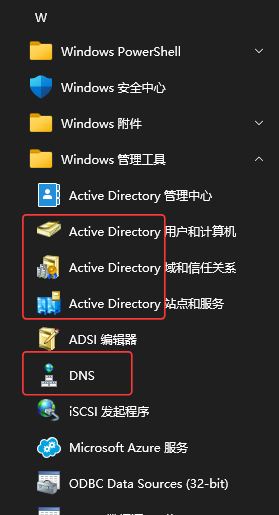
\includegraphics[width=0.72\textwidth]{img/dc_success.png}
    \caption{Windows Server 2022 成功升级为域控制器}
\end{figure}

随后在 Active Directory 用户和计算机中创建域用户，并通过委派控制向导为指定用户分配“将计算机加入到域”的相关控制权限。由图中可见，用户对象已经创建成功，且在控制委派过程中能够正确选定目标用户组，说明课堂实验要求中的“新建用户并选择将计算机加入到域”已经完成。

\begin{figure}[H]
    \centering
    \begin{minipage}{0.48\textwidth}
        \centering
        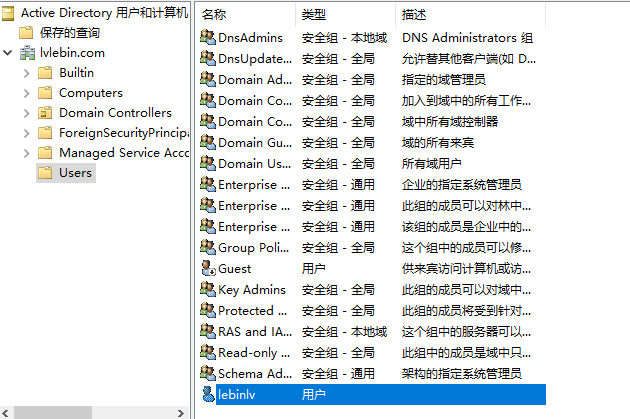
\includegraphics[width=\textwidth]{img/user_created.png}
    \end{minipage}
    \hfill
    \begin{minipage}{0.48\textwidth}
        \centering
        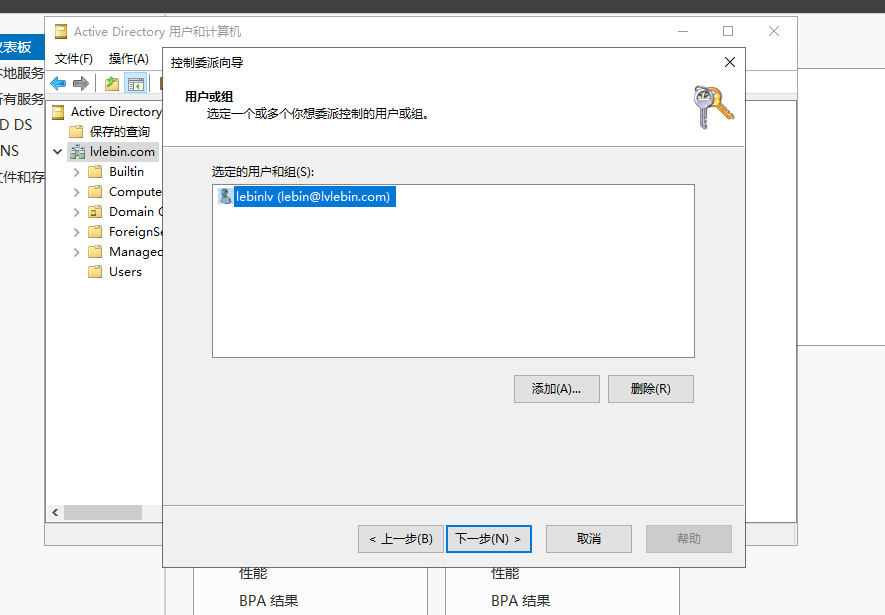
\includegraphics[width=\textwidth]{img/domain_delegate.png}
    \end{minipage}
    \caption{创建域用户并进行“将计算机加入到域”相关委派}
\end{figure}

在主机侧，将 Host-Only 网卡的首选 DNS 修改为域控制器地址 192.168.162.130，随后将主机加入到 lvlebin.com 域中。图中显示主机 DNS 已正确指向域控，且系统弹出“欢迎加入 lvlebin.com 域”的提示信息，说明 DNS 解析与加域过程正确完成。

\begin{figure}[H]
    \centering
    \begin{minipage}{0.30\textwidth}
        \centering
        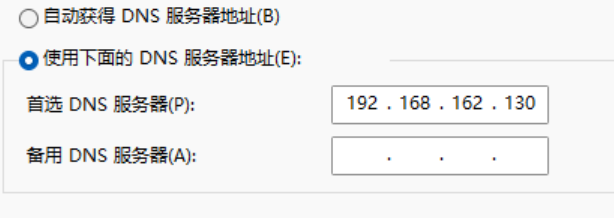
\includegraphics[width=\textwidth]{img/dns_changed.png}
    \end{minipage}
    \hfill
    \begin{minipage}{0.30\textwidth}
        \centering
        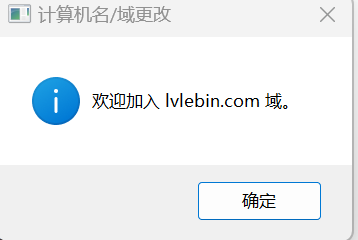
\includegraphics[width=\textwidth]{img/domain_join_success.png}
    \end{minipage}
    \hfill
    \begin{minipage}{0.30\textwidth}
        \centering
        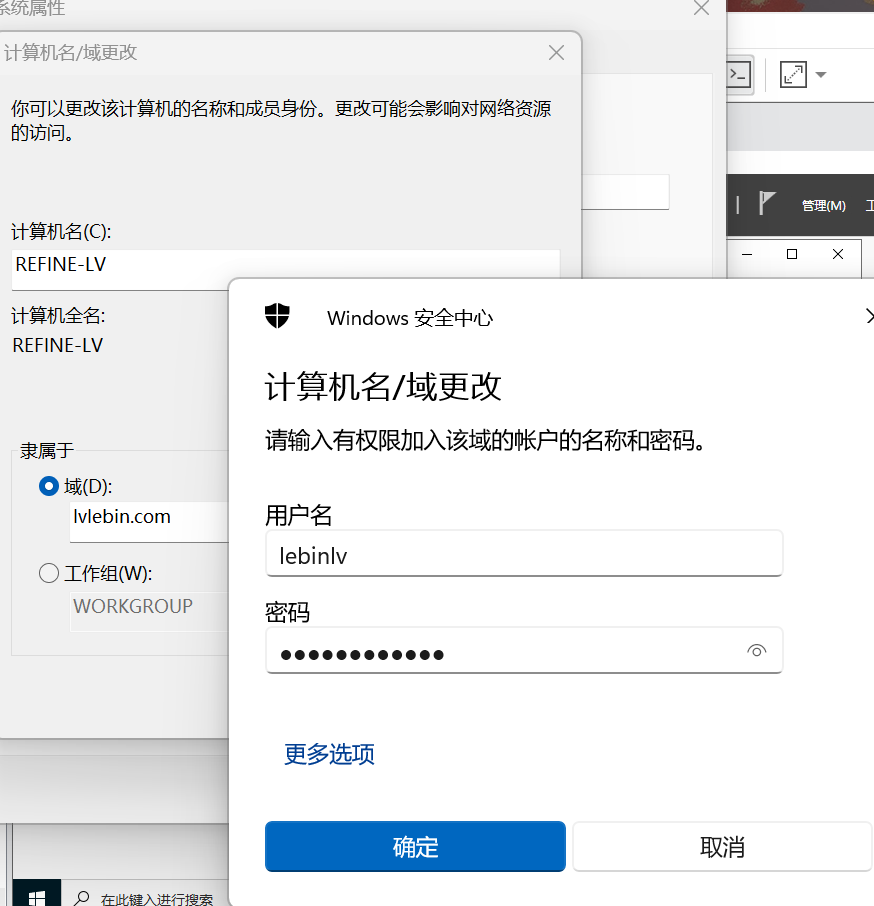
\includegraphics[width=\textwidth]{img/host_joined_domain.png}
    \end{minipage}
    \caption{主机修改首选DNS并成功加入自建域}
\end{figure}

完成加域后，在虚拟机与主机两侧的 Windows Defender 防火墙高级安全中创建连接安全规则，并将身份验证方式设置为 Kerberos。图中可见两端均已创建对应规则，表明课堂实验中的“分别在虚拟机和主机创建IP策略”要求已经满足。

\begin{figure}[H]
    \centering
    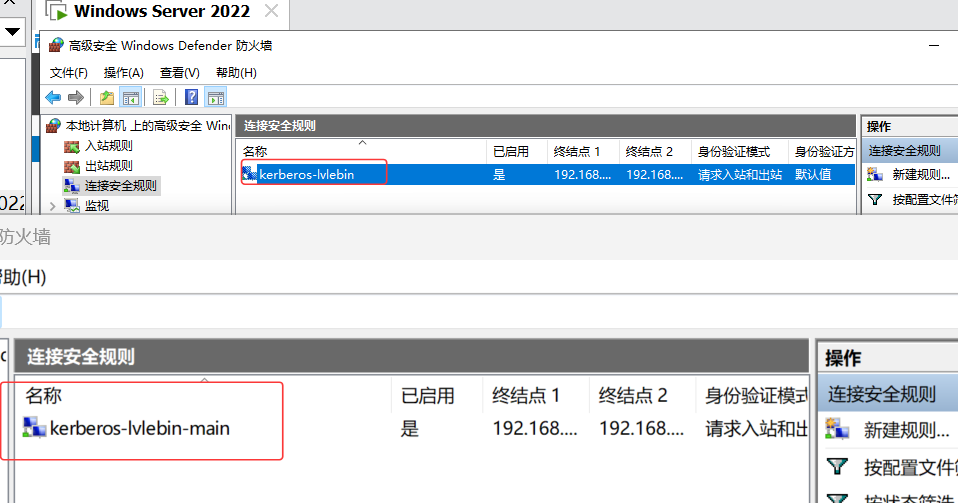
\includegraphics[width=0.90\textwidth]{img/ipsec_rules.png}
    \caption{虚拟机与主机分别创建基于 Kerberos 的连接安全规则}
\end{figure}

在策略生效后，主机成功 ping 通域控制器地址 192.168.162.130，说明网络连通正常。进一步使用 PowerShell 命令 Get-NetIPsecMainModeSA 分别在主机和虚拟机上查看安全关联信息，可以看到 LocalAddress、RemoteAddress、AuthenticationMethod、IntegrityAlgorithm、State 等字段均已正确显示，其中 AuthenticationMethod 为 Kerberos，IntegrityAlgorithm 为 SHA1，State 为 Active，说明 IPSec 主模式安全关联已经建立，课堂实验最终验证通过。

\begin{figure}[H]
    \centering
    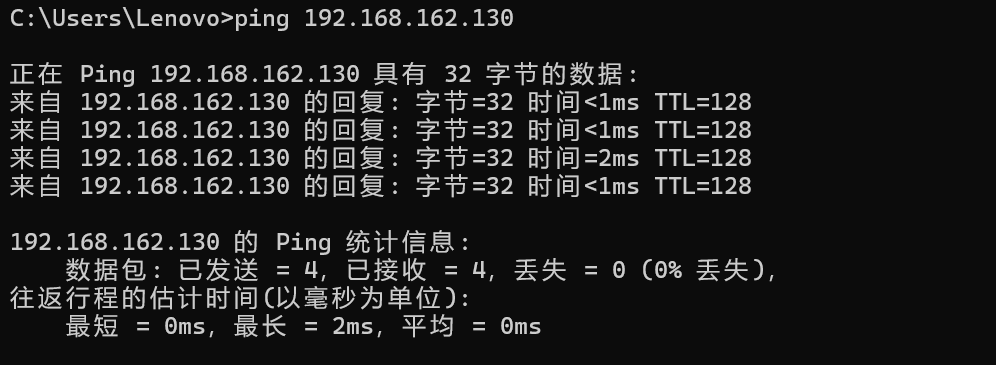
\includegraphics[width=0.78\textwidth]{img/ping_ok.png}
    \caption{主机成功与域控制器互相连通}
\end{figure}

\begin{figure}[H]
    \centering
    \begin{minipage}{0.49\textwidth}
        \centering
        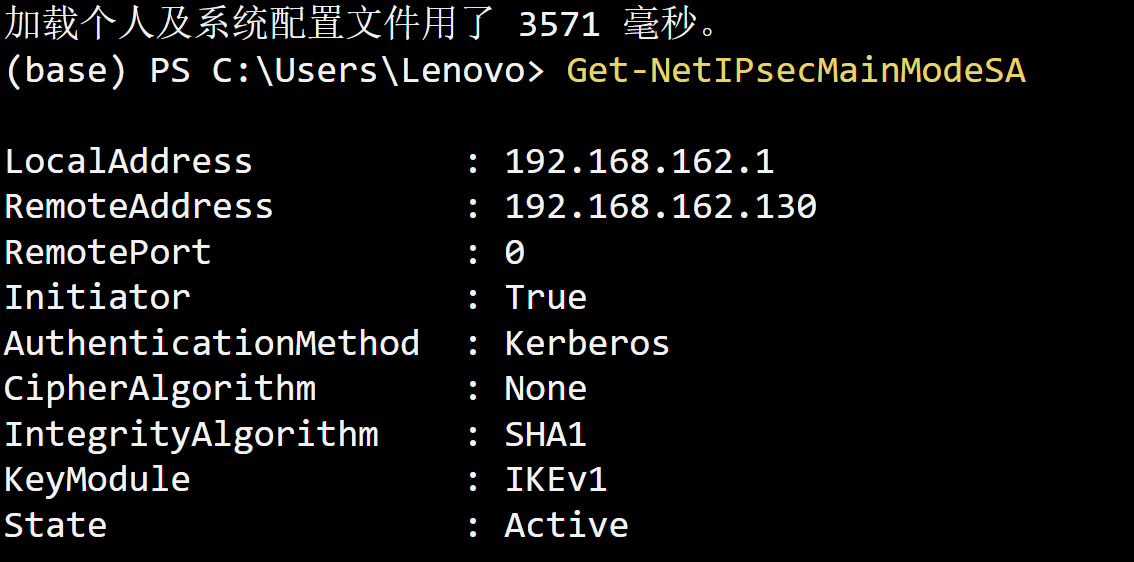
\includegraphics[width=\textwidth]{img/mainmode_host.png}
    \end{minipage}
    \hfill
    \begin{minipage}{0.49\textwidth}
        \centering
        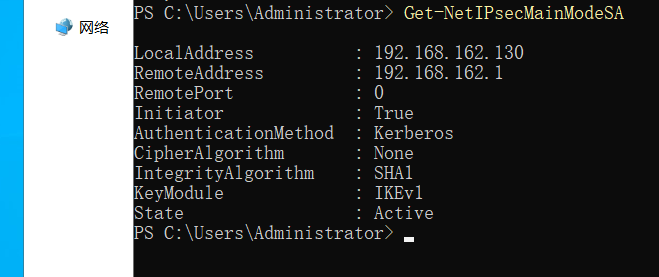
\includegraphics[width=\textwidth]{img/mainmode_server.png}
    \end{minipage}
    \caption{主机与虚拟机中 IPSec 主模式安全关联结果}
\end{figure}

综上，课堂实验中关于域控搭建、用户与加域配置、Kerberos 身份验证与 IPSec 安全关联建立的要求均已完成。

\subsection*{（二）实验一：Windows平台下配置Kerberos身份认证系统}
实验一要求在 Windows 平台下完成 Kerberos 身份认证系统配置。本实验在前期课堂实验与相关 Windows 域环境配置基础上，已经完成了域控制器部署、DNS 服务启用、用户创建以及客户端加入域等关键操作。因此，实验一在本次实验中主要体现为对已有环境的验证与总结，而不再重复完整搭建过程。

从结果上看，Windows Server 2022 已经作为域控制器运行，DNS 正常工作，客户端主机能够成功加入 lvlebin.com 域，并可使用域账户进行身份认证。这说明 Windows 平台下 Kerberos 身份认证系统已经搭建完成。其本质在于域控制器中运行的 KDC 为用户和服务签发票据，客户端通过域登录与后续访问过程实现 Kerberos 身份认证。

\begin{figure}[H]
    \centering
    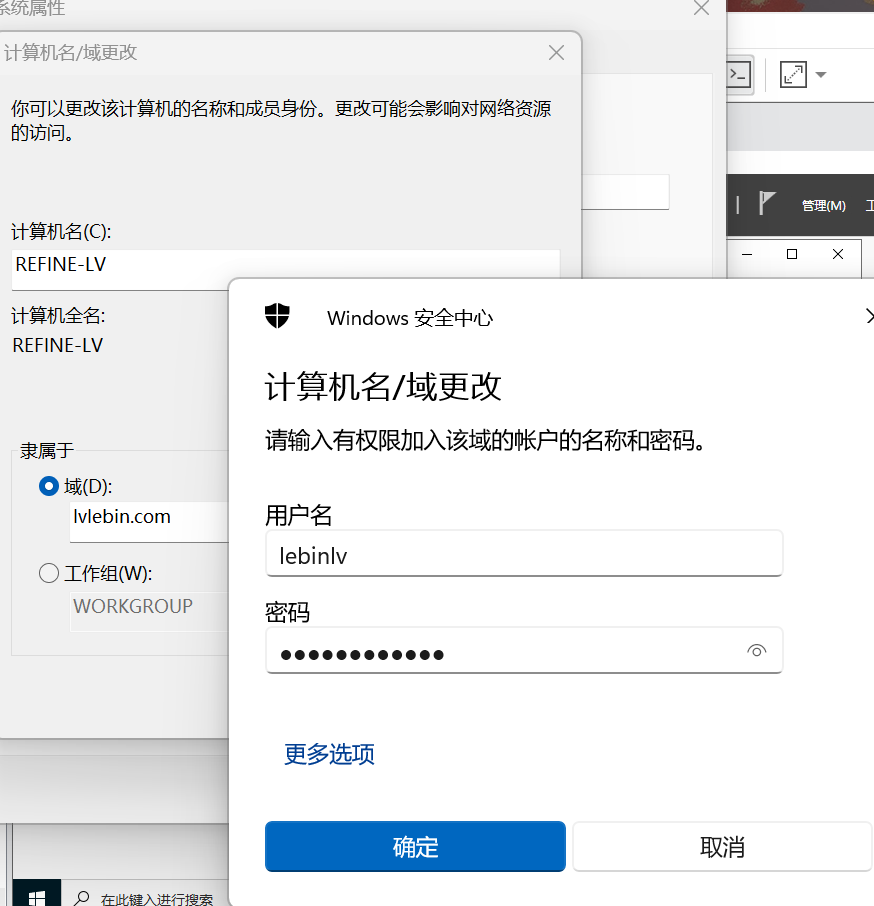
\includegraphics[width=0.48\textwidth]{img/host_joined_domain.png}
    \caption{实验一结果图：Windows 客户端成功加入域并完成身份认证环境配置}
\end{figure}

由此可见，Windows 平台 Kerberos 身份认证系统已经能够在当前实验环境中正常工作，为后续基于 Kerberos 的 IPSec 认证奠定了基础。

\subsection*{（三）实验二：Linux平台下配置Kerberos身份认证系统}
实验二在 Ubuntu 平台上完成 Kerberos 服务端与客户端环境的配置。首先安装 krb5-kdc、krb5-admin-server、krb5-user 等软件包，并在安装过程中设置 realm 为 LLBTEST.COM。随后按照实验要求对 Linux 平台中的 Kerberos 关键配置文件进行修改，主要包括 krb5.conf、kdc.conf 与 kadm5.acl。图中给出了 Linux 平台中配置过程的关键界面，说明实验环境已经完成基本参数设置。

\begin{figure}[H]
    \centering
    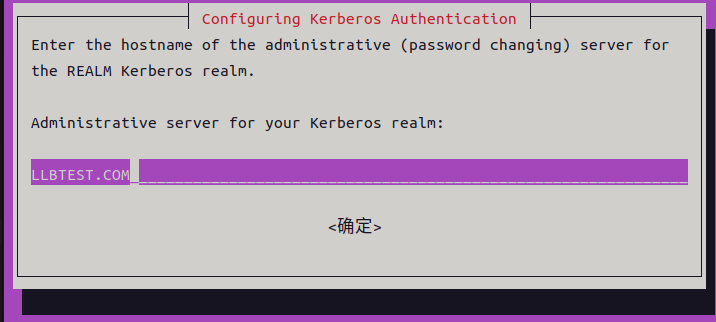
\includegraphics[width=0.62\textwidth]{img/linux_config.png}
    \caption{Ubuntu 平台中 Kerberos 配置过程界面}
\end{figure}

完成配置后，启动 krb5-kdc 和 krb5-admin-server 服务。系统状态显示 krb5-kdc 处于 active (running) 状态，表明 Linux 平台中的 KDC 已成功启动，具备向用户签发票据的能力。

\begin{figure}[H]
    \centering
    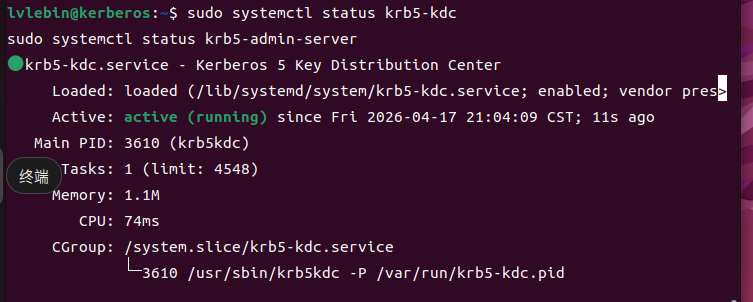
\includegraphics[width=0.76\textwidth]{img/linux_service.png}
    \caption{Kerberos 服务配置完成后成功启动}
\end{figure}

之后，在 KDC 中创建管理员 principal、普通用户 principal 以及服务 principal，并通过 kinit 获取用户 lebin@LLBTEST.COM 的票据。由 klist 输出可见，默认 principal 为 lebin@LLBTEST.COM，票据缓存中已存在 krbtgt/LLBTEST.COM@LLBTEST.COM，说明用户已经成功从 KDC 获取了初始票据，这也是 Linux 平台 Kerberos 身份认证系统配置成功的核心标志。

\begin{figure}[H]
    \centering
    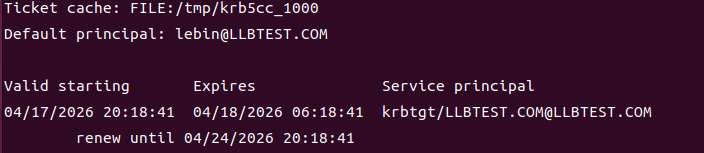
\includegraphics[width=0.76\textwidth]{img/linux_klist.png}
    \caption{使用 kinit 获取票据后通过 klist 查看票据缓存}
\end{figure}

进一步地，在服务 principal 基础上生成 keytab 文件，并使用 klist -k 查看 keytab 内容。图中显示 keytab 中已经包含 host/kerberos.test.com@LLBTEST.COM，对应服务端运行所需的身份信息，说明 Linux 平台 Kerberos 服务端认证环境也已经准备完成。

\begin{figure}[H]
    \centering
    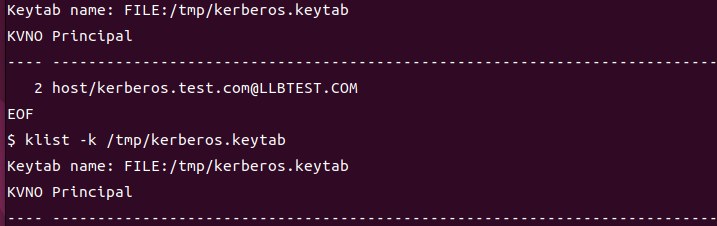
\includegraphics[width=0.76\textwidth]{img/linux_keytab.png}
    \caption{生成并查看服务端 keytab 文件内容}
\end{figure}

综上，实验二已经完成 Ubuntu 平台下 Kerberos 服务的部署、principal 的创建、票据的获取以及 keytab 的生成，表明 Linux 平台下的 Kerberos 身份认证系统配置成功。

\subsection*{（四）实验三：Kerberos客户端程序编程}
实验三要求参考 Kerberos 软件包中 simple/client 与 simple/server 的目录结构，自行编写代码替换其中的 c 文件与 h 文件，并通过 make 编译得到可执行程序。结合前述实验二已经建立好的 LLBTEST.COM Kerberos 环境，本实验编写了一个最小化的客户端程序和服务端程序：客户端负责读取当前票据缓存中的 principal，服务端负责读取 keytab 中保存的服务 principal，从而验证 Kerberos 客户端与服务端环境是否正常。

在程序运行结果中，服务端输出显示 keytab 路径为 FILE:/tmp/kerberos.keytab，且成功识别出服务 principal 为 host/kerberos.test.com@LLBTEST.COM，说明服务端已经能够正确访问 Kerberos keytab 文件并读取服务身份信息。

\begin{figure}[H]
    \centering
    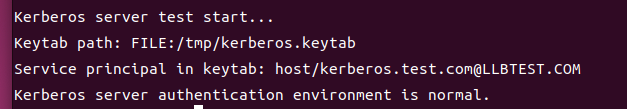
\includegraphics[width=0.76\textwidth]{img/exp3_server.png}
    \caption{实验三服务端程序运行结果}
\end{figure}

客户端输出则显示当前票据 principal 为 lebin@LLBTEST.COM，说明客户端能够读取当前 Kerberos 票据缓存，并确认用户票据已经存在。因此，客户端程序可认为已经完成了对当前 Kerberos 身份认证环境的验证。

\begin{figure}[H]
    \centering
    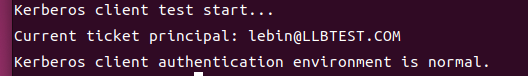
\includegraphics[width=0.76\textwidth]{img/exp3_client.png}
    \caption{实验三客户端程序运行结果}
\end{figure}

实验三虽然采用的是简化版客户端与服务端测试程序，但已经符合课程要求中“编制客户端程序使用 Kerberos 实现身份认证功能”的基本目标，能够从应用层面对票据缓存和服务端 keytab 进行读取与验证，体现了 Kerberos 在程序设计中的基本使用方式。
\\
{\heiti\zihao{4} 八、实验结论、心得体会和改进建议：}

通过本次 Kerberos 综合实验，可以较为系统地理解 Kerberos 协议在 Windows 和 Linux 平台中的实际部署过程，以及其在应用认证中的基本使用方式。课堂实验与实验一使我掌握了在 Windows 域环境中搭建 KDC、配置 DNS、创建域用户、将客户端加入域以及基于 Kerberos 配置 IPSec 连接安全规则的方法；实验二使我掌握了在 Ubuntu 平台中配置 krb5.conf、kdc.conf、kadm5.acl、初始化 KDC 数据库、创建 principal、获取票据以及生成 keytab 的基本流程；实验三则进一步说明，在完成 Kerberos 环境部署后，客户端与服务端程序可以利用票据缓存与 keytab 对身份认证环境进行应用层验证。

从实验结果来看，Kerberos 协议的核心优势在于能够利用 AS、TGS 和票据机制替代明文口令传输，实现基于可信第三方的安全身份认证。在 Windows 域环境中，Kerberos 与 Active Directory、DNS 和域控制器紧密结合，适合集中式用户管理与企业级网络认证；在 Linux 环境中，Kerberos 则表现为更加灵活的服务端和客户端配置过程，便于理解其底层工作机制。二者相互结合，使我对 Kerberos 的原理和实际部署方式都有了更清晰的认识。

在实验过程中，也存在一些值得改进的地方。首先，Windows 平台下 IPSec 安全关联在新系统界面中与旧版教材中的“IP 安全策略管理”存在一定差异，初学时容易在“请求身份验证”和“要求身份验证”等细节处出现理解偏差；其次，Linux 平台下 Kerberos 配置文件较多，对 realm、主机名、hosts 解析、服务状态等细节要求严格，任何一个参数不一致都可能导致 kinit 失败；最后，实验三中虽然已实现最小化程序验证，但如果后续有更充足的时间，可以进一步扩展为真正的客户端/服务端网络通信模型，使程序对 Kerberos 票据验证过程的体现更加完整。

总体而言，本次实验较完整地覆盖了 Kerberos 从协议原理到系统配置、再到程序验证的全过程，不仅加深了我对身份认证机制的理解，也提升了我在 Windows、Linux 以及应用层开发三个层面综合分析和解决问题的能力。

\newpage
\appendix
\section*{附录A\quad Kerberos\_Client主要源代码}

\begin{lstlisting}
#include <stdio.h>
#include <stdlib.h>
#include <krb5.h>
#include "client.h"

int run_client(void) {
    krb5_context ctx = NULL;
    krb5_ccache ccache = NULL;
    krb5_principal princ = NULL;
    char *name = NULL;
    krb5_error_code ret;

    ret = krb5_init_context(&ctx);
    if (ret) {
        fprintf(stderr, "krb5_init_context failed\n");
        return 1;
    }

    ret = krb5_cc_default(ctx, &ccache);
    if (ret) {
        fprintf(stderr, "krb5_cc_default failed\n");
        krb5_free_context(ctx);
        return 1;
    }

    ret = krb5_cc_get_principal(ctx, ccache, &princ);
    if (ret) {
        fprintf(stderr, "No valid Kerberos ticket cache found.\n");
        krb5_cc_close(ctx, ccache);
        krb5_free_context(ctx);
        return 1;
    }

    ret = krb5_unparse_name(ctx, princ, &name);
    if (ret) {
        fprintf(stderr, "krb5_unparse_name failed\n");
        krb5_free_principal(ctx, princ);
        krb5_cc_close(ctx, ccache);
        krb5_free_context(ctx);
        return 1;
    }

    printf("Kerberos client test start...\n");
    printf("Current ticket principal: %s\n", name);
    printf("Kerberos client authentication environment is normal.\n");

    krb5_free_unparsed_name(ctx, name);
    krb5_free_principal(ctx, princ);
    krb5_cc_close(ctx, ccache);
    krb5_free_context(ctx);

    return 0;
}

int main(void) {
    return run_client();
}
\end{lstlisting}

\section*{附录B\quad Kerberos\_Server主要源代码}

\begin{lstlisting}
#include <stdio.h>
#include <stdlib.h>
#include <krb5.h>
#include "server.h"

int run_server(void) {
    krb5_context ctx = NULL;
    krb5_keytab keytab = NULL;
    krb5_kt_cursor cursor;
    krb5_keytab_entry entry;
    krb5_error_code ret;
    char *name = NULL;

    const char *keytab_path = "FILE:/tmp/kerberos.keytab";

    ret = krb5_init_context(&ctx);
    if (ret) {
        fprintf(stderr, "krb5_init_context failed\n");
        return 1;
    }

    ret = krb5_kt_resolve(ctx, keytab_path, &keytab);
    if (ret) {
        fprintf(stderr, "krb5_kt_resolve failed: cannot open %s\n", keytab_path);
        krb5_free_context(ctx);
        return 1;
    }

    ret = krb5_kt_start_seq_get(ctx, keytab, &cursor);
    if (ret) {
        fprintf(stderr, "krb5_kt_start_seq_get failed\n");
        krb5_kt_close(ctx, keytab);
        krb5_free_context(ctx);
        return 1;
    }

    ret = krb5_kt_next_entry(ctx, keytab, &entry, &cursor);
    if (ret) {
        fprintf(stderr, "No keytab entry found in %s\n", keytab_path);
        krb5_kt_end_seq_get(ctx, keytab, &cursor);
        krb5_kt_close(ctx, keytab);
        krb5_free_context(ctx);
        return 1;
    }

    ret = krb5_unparse_name(ctx, entry.principal, &name);
    if (ret) {
        fprintf(stderr, "krb5_unparse_name failed\n");
        krb5_free_keytab_entry_contents(ctx, &entry);
        krb5_kt_end_seq_get(ctx, keytab, &cursor);
        krb5_kt_close(ctx, keytab);
        krb5_free_context(ctx);
        return 1;
    }

    printf("Kerberos server test start...\n");
    printf("Keytab path: %s\n", keytab_path);
    printf("Service principal in keytab: %s\n", name);
    printf("Kerberos server authentication environment is normal.\n");

    krb5_free_unparsed_name(ctx, name);
    krb5_free_keytab_entry_contents(ctx, &entry);
    krb5_kt_end_seq_get(ctx, keytab, &cursor);
    krb5_kt_close(ctx, keytab);
    krb5_free_context(ctx);

    return 0;
}

int main(void) {
    return run_server();
}
\end{lstlisting}

\section*{附录C\quad Makefile主要内容}

\begin{lstlisting}[language={}]
CC=gcc
CFLAGS=$(shell krb5-config --cflags krb5)
LIBS=$(shell krb5-config --libs krb5)

CLIENT_SRC=src/appl/simple/client/client.c
SERVER_SRC=src/appl/simple/server/server.c

all: client server

client: $(CLIENT_SRC)
	$(CC) $(CLIENT_SRC) -o client $(CFLAGS) $(LIBS)

server: $(SERVER_SRC)
	$(CC) $(SERVER_SRC) -o server $(CFLAGS) $(LIBS)

clean:
	rm -f client server
\end{lstlisting}

\end{document}